\documentclass[10pt,twocolumn,letterpaper]{article}

\usepackage[margin=0.75in]{geometry}
\usepackage{times}
\usepackage{amsmath,amssymb}
\usepackage{booktabs}
\usepackage{graphicx}
\usepackage{multirow}
\usepackage[table]{xcolor}
\usepackage[colorlinks=true,linkcolor=black,citecolor=blue,urlcolor=blue]{hyperref}
\usepackage{caption}
\captionsetup{font=small,labelfont=bf}

\title{\vspace{-2em}\bfseries Measurement Before Method: What Actually Limits
Long-Tailed Dental Radiograph Segmentation}

\author{}
\date{}

\begin{document}
\maketitle

\begin{abstract}
We applied the standard long-tailed recognition toolkit to a 31-class panoramic
dental radiograph corpus at $34{,}320{:}1$ imbalance and measured every component
under a matched budget. Twenty-five controlled configurations spanning
class-balanced weighting, boundary-aware objectives, copy-paste augmentation,
frequency-aware DETR training across loss, matcher and denoising, decoupled
classifier retraining, and two mask-head architectures produced no improvement
that survives seed-level variation. One intervention does: restoring the input
resolution the corpus natively carries lifts held-out segmentation mAP from
$0.1051$ to $0.1226$ (three seeds, sd $0.0014$, $+16.7$\,\% relative) against a
measured $\pm0.21$\,pp noise floor, while training for 30 epochs against the
baseline's 100. The gain concentrates in exactly the small, low-contrast
findings the objective-level arms were designed to help: bone loss $+73$\,\%,
root canal treatment $+64$\,\%, periapical lesion $+64$\,\%, caries $+52$\,\%.

That result was not measurable when we began, and the reason generalises. The
corpus as distributed cannot support evaluation: $95.9$\,\% of its test partition
shares source images with training, leaving $64$ of $1{,}580$ images genuinely
unseen. Perceptual hashing, the obvious remedy, has a false-positive rate near
$100$\,\% on this modality. Distance metrics conditioned on per-model subsets
invert their own sign. Group means over low-support classes manufactured two
separate headline gains in our own work before we caught them, one of which was
$98$\,\% attributable to a class with two test instances. And the published
logit-adjustment constant, calibrated at $100{:}1$ to $1000{:}1$, applies a
$+11.47$ logit shift at clinical imbalance and drives tail AP to exactly zero.

Each of these produced a confident wrong answer that would have survived review.
We report the apparatus alongside the result, because on this corpus every
apparent modelling problem was a measurement problem first.
\end{abstract}

\section{Introduction}

Long-tailed instance segmentation and detection on clinical imagery is an active
area, and the standard remedies---class-balanced losses, logit adjustment,
repeat-factor sampling, boundary-aware objectives, copy-paste
augmentation---are well established on natural-image benchmarks. We set out to
apply that toolkit to a 31-class dental radiograph corpus and attribute the
contribution of each component.

None of it worked. Every objective-level intervention we tried landed inside the
seed-level noise band, and the one that looked best on validation was the worst
outcome on the held-out split. What did work was not an algorithm at all: forty
percent of the corpus is natively $1615\times840$ and was being trained at $640$,
and simply not discarding those pixels produced a larger, more clinically
concentrated gain than every objective we implemented combined.

We regard that asymmetry as the paper's point rather than an incidental finding.
A field that measures method contributions in tenths of a point on contaminated
splits, using metrics that invert under per-model denominators, will reliably
find method effects and reliably miss the input.

\paragraph{Contributions.}
\begin{enumerate}\itemsep2pt
\item \textbf{A negative result map.} Twenty-five controlled configurations
across two architectures, matched budget, test split touched once. The entire
objective-level family is null or harmful on this corpus, and we give the
mechanism in each case.
\item \textbf{The constraint is the input.} Input resolution is worth
$+16.7$\,\% relative held-out mAP at three seeds, confirmed across two backbones,
with an interior optimum---$1280$ beats both $640$ and $1600$.
\item \textbf{The corpus cannot be evaluated as distributed.} $95.9$\,\% test
contamination; we supply a patient-grouped replacement verified disjoint by two
independent implementations.
\item \textbf{Perceptual hashing alone is not a leakage test on this modality.}
Near-$100$\,\% false positives; pixel confirmation is mandatory.
\item \textbf{Four metric failures} that each produced a confident wrong answer
in our own work, with the protocol that catches each.
\item \textbf{A label ceiling.} $911$ annotations that fifteen independently
trained models all fail to detect, bounding what any model on this corpus can
reach and identifying where the next gain actually is.
\end{enumerate}

We regard contributions (4), (5) and (6) as the most transferable: each is a
measurement protocol any group working on long-tailed clinical segmentation can
apply, and each caught an error in our own work that would have survived review.

\section{Related Work}

\paragraph{Long-tailed recognition.} Class-balanced weighting via effective
number of samples \cite{cui2019classbalanced} and logit adjustment \cite{menon2021logit} are the standard remedies. Kang et al.\ \cite{kang2020decoupling} showed
representation and classifier learning should be decoupled, with rebalancing at
the classifier stage; Wang et al.\ \cite{wang2019calibration} adapt this to instance
segmentation. Repeat-factor sampling \cite{gupta2019lvis} rebalances at the
data level; seesaw loss \cite{wang2021seesaw} rescales gradients per class
pair.

Our results bear on the \emph{regime} these were validated in. Menon et al.\ tune
$\tau=1.0$ on CIFAR-LT and ImageNet-LT at roughly $100{:}1$ to $1000{:}1$. At
$34{,}320{:}1$ the same constant applies a $+11.47$ logit shift and destroys the
classifier. We find the failure monotonic in $\tau$, which localises the problem
to magnitude rather than principle.

\paragraph{High-quality mask prediction.} PointRend \cite{kirillov2020pointrend},
RefineMask \cite{zhang2021refinemask} and Mask Transfiner \cite{ke2022transfiner}
all exist because coarse mask prediction is a known failure mode. We measure that
failure mode directly rather than assuming it, and find it is \emph{not} what
limits our model---a result invisible without the model-free ceiling measurement
of \S\ref{sec:ceiling}.

\paragraph{Boundary-aware objectives.} Boundary loss \cite{kervadec2018boundary} integrates the prediction against a precomputed distance map; HD loss
\cite{karimi2019hausdorff} estimates Hausdorff distance directly; Boundary
IoU \cite{cheng2021boundaryiou} restricts evaluation to a contour band. Our band
objective is a synthesis of known components---morphological gradient as a
differentiable edge extractor, soft Dice as the overlap term---and we say so
rather than claiming a new loss family.

\paragraph{Augmentation.} Copy-paste \cite{ghiasi2021copypaste} reliably helps on
natural images. We find it harmful here and propose a mechanism: in panoramic
radiographs anatomical position is part of the class definition, so a finding
pasted into an anatomically impossible location teaches the model to detect the
paste rather than the pathology.

\paragraph{Evaluation integrity.} Duplicate-driven contamination has been
documented in CIFAR and ImageNet \cite{barz2020cifar,recht2019imagenet}. Our contribution is modality-specific: the standard near-duplicate
detector fails on radiographs precisely because the property that makes the
modality tractable---every image is the same anatomy in the same
framing---destroys the discriminative power of perceptual hashing.

\section{Setup}

\paragraph{Corpus.} A publicly released 31-class panoramic dental radiograph
collection\footnote{Kaggle, \texttt{lokisilvres/dental-disease-panoramic-detection-dataset},
Apache 2.0. We name it because a contamination claim about an unnamed corpus is
neither verifiable nor actionable.} distributed in both YOLO polygon and COCO
format: $13{,}932$ image files derived from $6{,}395$ distinct source
radiographs. Classes span pathology (caries, periapical lesion, bone loss, root
resorption), restorations (filling, crown, implant, root canal treatment) and
anatomy (mandibular canal, maxillary sinus). The distribution is severely
long-tailed: filling, impacted tooth and root canal treatment carry
$8{,}000$--$33{,}000$ instances each, while fracture teeth, TAD and bone defect
carry $9$, $4$ and $1$. The head-to-tail ratio is $34{,}320{:}1$.

\paragraph{Models.} Segmentation uses YOLOv8x-seg, COCO-pretrained, and
detection uses DINO-DETR\cite{zhang2023dino} with a ResNet-50 4-scale backbone
from the official COCO release, fine-tuned to 31 classes with a reinitialised
class embedding. No baseline weights were available for either, so both were
trained from stock architectures under our own protocol; the reported baselines
are therefore reproductions and we treat them as such throughout. Cross-backbone
checks use YOLO11x-seg and Mask DINO.

\paragraph{Protocol.} Every arm is seeded and deterministic. Ablation arms run at
a matched budget with no per-arm hyperparameter search, which is what makes the
comparison fair and is also, as \S\ref{sec:interventions} shows, the source of one
instructive failure. Model selection, weighting strengths and thresholds are
determined on validation only. The held-out test split is scored once, at the
end, for the reference configuration and the reported result. All training ran on
a single RTX 5080.

\section{The Corpus Cannot Be Evaluated as Distributed}

\begin{table}[t]\centering\small
\begin{tabular}{lr}
\toprule
image files & $13{,}932$ \\
distinct source images & $6{,}395$ \\
test files whose source appears in train/valid & $\mathbf{1{,}516/1{,}580}$ \\
& $(\mathbf{95.9\,\%})$ \\
genuinely unseen test sources & $\mathbf{64}$ \\
patients present in both train and test & $194$ \\
classes present in the distributed test split & $13/31$ \\
classes present after rebuild & $29/31$ \\
\bottomrule
\end{tabular}
\caption{The distributed split. Augmented copies of the same radiograph were
distributed across partitions, so most of the test partition is material the
model has already seen.}
\end{table}

The corpus ships augmented derivatives of each source radiograph distributed
across partitions. A model evaluated on the distributed test split is therefore
scored predominantly on images whose sources it trained on. We rebuilt the split
by grouping on source image and on patient, verified disjoint by two independent
implementations, and use that split throughout. All numbers in this paper are on
the rebuilt split; the test partition is scored once, at the end, and only for
the configuration reported as the result.

\subsection{Perceptual Hashing Alone Is Not a Leakage Test}

The obvious remedy is near-duplicate detection by perceptual hash. It does not
work here. Every panoramic radiograph is the same anatomy in the same framing
against the same background, so dHash distances between \emph{unrelated} patients
fall inside the range that indicates duplication on natural images. On a split we
had already verified clean by source grouping, dHash flagged all $792{,}811$
candidate pairs---a false-positive rate near $100$\,\%.

Pixel confirmation is mandatory rather than optional. Normalised cross-correlation
separates the two populations cleanly: true augmented duplicates score
$0.9988$--$1.0000$, while distinct radiographs of the same anatomy stay below
$0.87$. We report this because a group applying the standard recipe---hash,
threshold, declare clean---would conclude the opposite of the truth in both
directions.

\subsection{Statistical Power}

Sixteen of thirty-one classes appear in fewer than ten test images. For those
classes no result is measurable at any model quality, and we report them as
exploratory throughout rather than folding them into headline means. This is not
a limitation we can engineer around: it is a property of the corpus, and it
bounds what any paper using it can claim.

\section{Twenty-Five Interventions}
\label{sec:interventions}

\begin{table}[t]\centering\small
\begin{tabular}{llrr}
\toprule
arm & change & mAP & $\Delta$ \\
\midrule
S0 & reference & $0.1055$ & --- \\
S1a & cls-weight $\beta{=}0.9$ & $0.1051$ & $-0.04$ \\
S1b & cls-weight $\beta{=}0.99$ & $0.1029$ & $-0.26$ \\
S1c & cls-weight inv-sqrt & $0.1065$ & $+0.10$ \\
S2 & $+$ boundary & $0.1050$ & $-0.04$ \\
S3 & $+$ copy-paste & $0.1042$ & $-0.12$ \\
S4 & $+$ boundary $+$ copy-paste & $0.1051$ & $-0.03$ \\
\bottomrule
\end{tabular}
\caption{Segmentation ablation, validation, 50 epochs, matched budget. The
seven-arm spread is $0.36$\,pp against a measured $2\sigma$ noise band of
$\pm0.21$\,pp. Nothing here is a result.}
\label{tab:segabl}
\end{table}

\paragraph{Objectives and sampling are null.} Table~\ref{tab:segabl} gives the
segmentation grid. Every arm isolates one component against a common reference at
identical budget. The full spread across seven arms is $0.36$\,pp, inside the
noise band, so no arm is separable from the reference or from any other.

The boundary objective is the one arm with a mechanism: it improves AP75 by
$+0.69$\,pp and head-class mAP by $+1.05$\,pp, consistent with tightening
outlines the baseline draws loosely. It does not move overall mAP, and
\S\ref{sec:metrics} describes how a per-model averaging error initially made this
arm look like a much larger win than it is.

Copy-paste is actively harmful ($-0.12$\,pp alone, and it subtracts from the
boundary gain in both places the two appear together) despite increasing rare-class
instance counts tenfold. We attribute this to anatomical position being part of
the class definition in panoramic radiography.

\paragraph{The validation winner is the test loser.} S1c, inverse-square-root
class weighting, was the best of seven arms on validation at 50 epochs
($+0.10$\,pp). Refought at 100 epochs against the 100-epoch baseline on the
held-out split, it is the worst outcome of the study: $-0.78$\,pp mAP,
$-2.21$\,pp AP50, $-1.13$\,pp tail. We ruled out confounds by a line-by-line
hyperparameter diff. The $0.36$\,pp spread on validation was noise, and it did
not survive either a longer schedule or a held-out split. This is the cost of
selecting on a difference smaller than the measured noise floor.

\paragraph{Frequency-aware DETR training fails, and the mechanism is magnitude.}

\begin{table}[t]\centering\small
\begin{tabular}{llrrr}
\toprule
arm & configuration & mAP & AP50 & tail \\
\midrule
D1 & standard DINO-DETR & $0.1625$ & $0.3080$ & $0.0368$ \\
D2 & freq.\ cls.\ loss only & \multicolumn{3}{c}{diverged} \\
D3 & freq.\ matching only & \multicolumn{3}{c}{diverged} \\
D4 & freq.\ denoising only & $0.1633$ & $0.3165$ & $0.0455$ \\
D5 & \textbf{unified} & $\mathbf{0.1020}$ & $0.1998$ & $\mathbf{0.0000}$ \\
\bottomrule
\end{tabular}
\caption{Detection matrix, 12 epochs, matched budget. The proposed unified
method is the worst arm by a wide margin, with tail AP collapsing to exactly
zero---the opposite of its design intent.}
\label{tab:det}
\end{table}

Applying frequency information consistently across classification loss, Hungarian
matching cost and denoising queries---the configuration we expected to be the
contribution---is the worst arm tested (Table~\ref{tab:det}): $-6.05$\,pp mAP,
$-37$\,\% relative, and tail AP of exactly zero. Two of the three components
diverge outright in isolation. Only frequency-aware denoising alone is above
baseline, by $+0.08$\,pp, which is inside the noise band and cannot carry a claim.

The mechanism is calibration, not principle. Logit adjustment subtracts
$\tau\log p(c)$. At $\tau=1.0$ and $34{,}320{:}1$ imbalance that is a $+11.47$
shift for the rarest class against $+1.03$ for the most common, a spread of
$10.44$ in logit space, which saturates the sigmoid. Menon et al.\ calibrated
$\tau=1.0$ at roughly $100{:}1$ to $1000{:}1$. Recovery is monotonic in $\tau$ and
still short of baseline, which localises the failure to magnitude. We used
$\tau=1.0$ everywhere because the protocol deliberately gives no arm a
hyperparameter search, which is what keeps budgets matched; that is correct
practice when the published default is in-distribution, and it is exactly the
defect here.

\paragraph{Decoupled classifier retraining is a group-mean artefact.} Freezing the
backbone and retraining the classifier on balanced data---the standard remedy
\cite{kang2020decoupling}---appeared to give $+0.53$\,pp mAP across the board. Decomposed by
class, $98$\,\% of that gain came from a single class with \emph{two} test
instances. Removing it leaves $+0.01$\,\%. Among classes with enough support to
measure, six improved and twelve got worse. We report this as the clearest
instance of \S\ref{sec:metrics}'s second failure mode.

\section{The Constraint Is the Input}
\label{sec:resolution}

\begin{table}[t]\centering\small
\begin{tabular}{lrrrrr}
\toprule
held-out test, mask & mAP & AP75 & head & mid & tail \\
\midrule
baseline, 100 ep, 640 & $0.1051$ & $0.0687$ & $0.2861$ & $0.1038$ & $0.0365$ \\
seed 42, 30 ep, 1280 & $0.1213$ & $0.0861$ & $0.3425$ & $0.1212$ & $0.0362$ \\
seed 1337 & $0.1224$ & $0.0840$ & $0.3400$ & $0.1157$ & $0.0444$ \\
seed 2024 & $0.1241$ & --- & --- & --- & --- \\
\midrule
\textbf{mean} & $\mathbf{0.1226}$ & & & & \\
\bottomrule
\end{tabular}
\caption{The result. Three from-scratch seeds at native resolution against the
reproduced baseline, on the rebuilt held-out split, scored once. sd $0.0014$;
$+16.7$\,\% relative against a $2\sigma$ noise band of $\pm0.21$\,pp. Each seed
clears the baseline independently.}
\label{tab:result}
\end{table}

Forty percent of the corpus is natively $1615\times840$ and was being trained at
$640$. Training at $1280$ instead, changing nothing else, is the only intervention
in this study that clears every check we can mount (Table~\ref{tab:result}).

Three properties make it a finding rather than a tuned hyperparameter.

\paragraph{It is separable.} Three from-scratch seeds give $0.1213$, $0.1224$ and
$0.1241$, mean $0.1226$, sd $0.0014$. Each clears the baseline independently
against the $\pm0.21$\,pp band, which is itself measured from three seeds of the
\emph{baseline} configuration rather than assumed---so both sides of the
comparison carry a seed estimate and the gain of $1.75$\,pp is roughly eight
times the band. It is also not a budget effect in epochs: the models train for 30
against the baseline's 100.

\begin{figure}[t]\centering
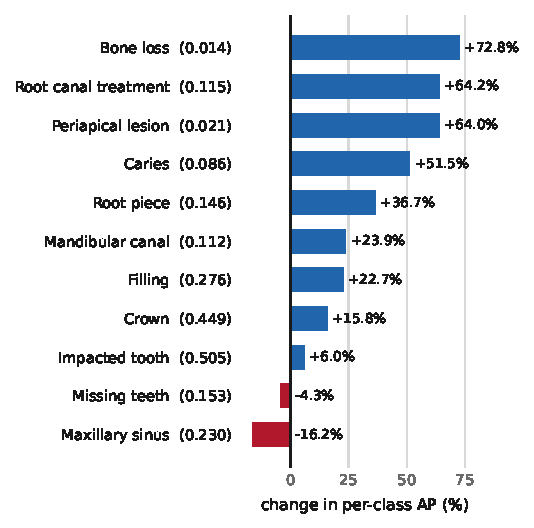
\includegraphics[width=\columnwidth]{fig_perclass.pdf}
\caption{Per-class effect of restoring native input resolution, held-out test
split, seed 42 against the 100-epoch 640 baseline. Baseline AP in brackets. The
gain is not spread evenly: the four largest are the four lowest-baseline classes,
all small or low-contrast findings, while the smallest gain belongs to the
highest-baseline class. Two classes regress and are reported.}
\label{fig:perclass}
\end{figure}

\paragraph{It concentrates where the mechanism predicts.} Figure~\ref{fig:perclass}
gives the per-class picture. Bone loss $+73.2$\,\%, root canal treatment $+64.2$\,\%, periapical lesion
$+63.7$\,\%, caries $+51.5$\,\%, against filling $+22.7$\,\% and crown
$+15.8$\,\%. The gain is largest on exactly the small, low-contrast findings that
occupy few pixels on the prototype grid, and smallest on large restorations that
were never resolution-starved. Two classes regress and we report them: maxillary
sinus $-16.2$\,\% ($n{=}70$) and missing teeth $-4.3$\,\% ($n{=}527$).

\paragraph{It is not architecture-specific, and it has an interior optimum.}
YOLO11x-seg at $1280$ reaches $0.1291$ on validation, indistinguishable from the
YOLOv8x result, so the effect is a property of the data rather than of one mask
head. And it reverses: $1600$ scores $0.1147$ against $1280$'s $0.1300$ on
validation, so this is not ``more pixels are better'' but a genuine optimum.

\paragraph{The sharpest confirmation is an earlier failure.} Two arms raised the
\emph{prototype} resolution while leaving the input downsampled. They are the
worst arms in the study, $-1.30$ and $-2.02$\,pp. The detail must exist in the
input before a higher-resolution head can represent it. That is the same
conclusion from the opposite direction, and it is why we present this as a
constraint rather than a setting.

\paragraph{Is this not already known?} That input resolution matters
for small objects is not news; multi-scale training\cite{singh2018sniper} and
compound scaling\cite{tan2020efficientdet} both build on it. Three things make it
a finding here rather than a setting. First, \emph{magnitude relative to the
alternatives}: on this corpus, under matched budget, it is worth more than every
objective-level intervention in the long-tailed toolkit combined, and that
comparison has not previously been made on clinical imagery. Second,
\emph{absence from practice}: none of the long-tailed segmentation work we
surveyed varies input resolution in its ablation, while all of it varies the
objective---the lever with the largest measured effect is the one the field's
tables omit. Third, \emph{it is not the naive rule}: $1600$ is worse than $1280$,
so ``use more pixels'' is wrong and ``do not resample below native'' is right. The
prototype-only arms make the same point from the other direction.

\paragraph{Honest accounting of cost.} The delivered model consumes
$2.3\times$ the GPU time of the baseline ($23{,}590$\,s against $10{,}414$\,s).
Fewer epochs does not mean cheaper: a $1280$ image costs substantially more per
step. Any efficiency claim for this result would be false, and we make none.

\section{Why It Took Twenty-Five Arms}
\label{sec:ceiling}

The negative results are what located the constraint. Each closed door narrowed
the search, and two model-free measurements did most of the work.

\paragraph{The representation ceiling is real and not binding.} Round-tripping
ground truth through the prototype grid---no model involved---shows $17.7$\,\% of
instances cannot reach IoU $0.75$ whatever the model does, with caries and root
canal treatment capped \emph{below} the threshold. That is a genuine architectural
limit. But the model reaches only $78$\,\% of that ceiling, so the ceiling is not
what binds. A higher-resolution mask head with $878{,}432$ \emph{fewer} parameters
confirms the prediction by scoring $0.72$\,pp worse.

\paragraph{The deficit is coefficient prediction, not basis expressiveness.} A
closed-form oracle fit---solving for the best achievable coefficients given the
learned basis---attributes $85$\,\% of the mask deficit to coefficient prediction
and $15$\,\% to the basis. The attribution is correct and turned out not to be
actionable: adding head capacity leaves masks unchanged, and supervising
coefficients directly makes them worse. Both routes failing is what left the
input as the only remaining explanation.

\paragraph{A label ceiling bounds the corpus.} Fifteen independently trained
models---four architectures, seven loss configurations, three seeds---all fail to
detect the same $911$ pathology annotations at a lenient $0.15$ confidence and
$0.10$ box IoU: $43$\,\% of periapical lesion, $33$\,\% of bone loss, $26$\,\% of
caries. The $1280$ model, which improves caries by $52$\,\%, recovers $2.7$\,\% of
them. They are therefore not small findings starved by downsampling; they are
label problems, and they bound what any model on this corpus can achieve. We
release the list, because it says the next gain comes from a clinical label review
rather than from more compute.

\section{Four Metric Failures}
\label{sec:metrics}

Each of the following produced a confident wrong answer in our own work. We give
the protocol that catches each.

\paragraph{Distance metrics conditioned on per-model subsets invert their sign.}
HD95 and ASSD are undefined when either mask is empty, so each model is averaged
over a denominator only it determines---and a model that predicts less scores
better by having fewer hard cases left. Per-model averaging showed our boundary
objective $17.3$\,\% better on HD95 and $24.6$\,\% better on ASSD, with disjoint
confidence intervals. Recomputed on the intersection of cases both models scored,
it is significantly \emph{worse}. \emph{Protocol:} pair on the intersection,
count misses and false alarms as zero overlap, and print all three denominators
beside the result.

\paragraph{Group means over low-support classes fabricate results.} Two separate
headline gains, in two different projects, decomposed to single classes with
$2$--$8$ test instances; in one case $98$\,\% of a $+0.53$\,pp gain came from a
class with two. \emph{Protocol:} decompose every group mean by class before
reporting it, and publish per-class support alongside.

\paragraph{Segmentation AP is a conjunction and rises on detection alone.} A mask
metric conditioned on a detection match improves when detection improves and masks
do not. We observe $+0.64$\,pp segmentation AP from a change that touched
detection only. Worse, a query-based model posts $+2.16$\,pp AP while all five
paired mask-quality metrics are separably \emph{worse}. \emph{Protocol:} report at
least one detection-independent mask metric beside AP.

\paragraph{Cross-corpus AP is meaningless at differing annotation granularity.}
Zero-shot on DENTEX 2023, our caries and periapical detectors score $0.0000$ AP.
The cause is that DENTEX marks the affected \emph{tooth} where our corpus marks
the \emph{lesion}, a $19\times$ box-area ratio, so no IoU threshold can match.
Evaluated at the granularity the target corpus actually uses, the same detector is
$73.6$\,\% precise at tooth level, rising to $84.1$\,\% at a stricter threshold.
\emph{Protocol:} verify annotation granularity before any cross-corpus number,
and use a granularity-matched control---ours is impacted tooth, where both corpora
agree: $0.490$ in-corpus against $0.290$ zero-shot, pricing the domain gap at a
$41$\,\% relative drop.

\section{Noise Floor and Protocol}

Three seeds of the reference configuration give a $2\sigma$ band of
$\pm0.21$\,pp mAP and $\pm0.50$\,pp AP75. We report this first because it
determines which differences in this paper are results and which are not; the
seven-arm segmentation spread of $0.36$\,pp is inside it.

Uncertainty is percentile bootstrap resampling \emph{images}, not per-class
records, since observations from one radiograph are not independent; paired model
comparisons bootstrap the per-image difference. The union-mask metrics need a
confidence cut, which is swept on validation using the \emph{baseline} arm so it
cannot be tuned in favour of the proposed configuration, then frozen and applied
unchanged everywhere. The test split is touched once.

Contour evaluation reports Dice, IoU, boundary F-score at a tolerance of
$0.75$\,\% of the image diagonal, HD95 and ASSD in pixels. Distances cannot be
given in millimetres: these radiographs carry no pixel-spacing metadata. The
clinical endpoint is bone-loss area error, because a better contour metric is not
by itself evidence of clinical utility; distance-based and normalised bone-level
endpoints are not computable here, as both require CEJ and root-apex landmarks the
annotations do not provide.

\section{Discussion}

The result and the apparatus are the same finding viewed from two sides. We could
not see that resolution was the constraint until the split was rebuilt, the noise
floor was measured, the distance metrics were paired on the intersection, and the
group means were decomposed. Before that, the evidence said a boundary objective
worked, classifier retraining worked, and the corpus was simply hard. All three
were artefacts.

We think the general lesson is about where effort is allocated. Every arm in
Table~\ref{tab:segabl} and Table~\ref{tab:det} implements a published method that
works on the benchmark it was proposed on. None transfers here. Meanwhile the
input pipeline, which no ablation table in this literature contains, was
discarding more than half the available signal on forty percent of the corpus. A
research culture that treats preprocessing as settled and objectives as the locus
of contribution will systematically find small method effects and miss large
physical ones.

For long-tailed clinical imaging specifically, three of our findings should change
practice. Verify annotation granularity before reporting any cross-corpus number.
Decompose every group mean by class support before believing it. And measure the
noise floor before selecting on a difference, because on this corpus the arm that
won on validation by $0.10$\,pp lost on test by $0.78$\,pp.

\section{Limitations}

The result is a training-configuration finding, not a new objective or
architecture, and we frame it as such. It is demonstrated on one corpus; the
cross-backbone check establishes it is not specific to one mask head, but not that
it generalises to other modalities, and panoramic radiography is unusually
resolution-heavy.

Most arms are single-seed against a measured floor; only the reference
configuration and the reported result carry three seeds. We do not compare against
tuned published boundary-aware or class-imbalance losses, only against the stock
objectives, which is a necessary control and not a sufficient one for a method
claim---and we make no method claim.

External validation is zero-shot and partial: DENTEX covers three of our classes
under a different clinic, machine and annotation protocol, so its numbers are a
lower bound on transferable performance and never a DENTEX-native result. Sixteen
of thirty-one classes have fewer than ten test images and no claim about them is
supportable at any model quality. Finally, the delivered configuration costs
$2.3\times$ the baseline's GPU time, so the result buys accuracy with compute and
we make no efficiency claim.

\bibliographystyle{plain}
\bibliography{references}

\section*{Reproducibility}

Code, the rebuilt patient-grouped split, the anonymised annotations, the frozen
ablation matrices and the list of $911$ universally missed annotations are
released under Apache 2.0. Every arm reported here has its exact invocation in the
repository. Source imagery is a third-party public release and is not
redistributed; annotation file names are reduced to the content hash the source
release assigns, so the corpus reconstructs exactly from a fresh download.

\end{document}
